\lstset{language=C}

\chapter{Loop Dependence Analysis}
\label{chap:dependencies}

\begin{quote}
  \emph{This chapter is adapted with permission from the PMPH Lecture
    Notes written by Cosmin Oancea.}
\end{quote}

So far, we have assumed that the user writes a fresh implementation of
a known algorithm, and that it can be straightforwardly expressed as
fully parallel loops, or as a simple reduction.  However, there is a
lot of legacy sequential scientific code written in imperative
languages such as C++, Java, Fortran, and either the precise algorithm
to which they correspond to (i) may have been forgotten (not
documented), or (ii) a fresh implementation is infeasible (e.g.,
because it costs too much).  At some point you may wish (or be asked)
to parallelise such code to run efficiently on a certain hardware.

This will require you to:

\begin{enumerate}
\item Identify the loop nests\footnote{A \emph{loop nest} is a
    collection of multiple loops nested within each other.} where most
  of the runtime is spent.

\item Parallelise these loops by reasoning at a low level of
  abstraction about which loops in the nest are parallel.

\item Decide on the manner in which loop nests can be re-written in
  order to optimise locality of reference, load balancing, thread
  divergence, etc.
\end{enumerate}

The main source of inspiration for the material presented in this and
\cref{chap:loop-transformations} has been the book ``Optimizing
compilers for modern architectures: a dependence-based
approach''~\cite{kennedy2001optimizing}.

This chapter is organised as follows:
\begin{itemize}
\item \Cref{sec:dir-vct} introduces various nomenclature,
  in particular the notion of cross-iteration dependency, and
  it shows how to summarise dependencies across the iteration
  space into a succinct representation, named direction vectors,
  that promotes reasoning about various code transformations.
\item \Cref{sec:loop-par} presents a simple theorem that allows easy
  identification of loop-level parallelism.
\end{itemize}

\section{Direction vectors}
\label{sec:dir-vct}

We start by defining the various reasons why a program statement must
be executed after some previous.  C executes statements in
\emph{program order}---the order they occur in the source code.
Dependence analysis is about distinguishing when the program order is
crucial for correct execution, and in which cases it is arbitrary
because C requires us to write statements in \emph{some} order.  If a
statement $S_{2}$ \emph{depends} on $S_{1}$, then $S_{2}$
must always be executed after $S_{1}$.  Dependencies typically
arise because the two statements interact with the same values, with
at least one of the statements changing the value.  When two
statements are not dependent on each other, they can in principle be
executed in parallel.  Our goal is to use dependence analysis to
identify when entire \emph{loop iterations} are independent, which
means that they can be executed in parallel.

\begin{figure}
  \centering
  \begin{subfigure}[t]{0.32\textwidth}
\begin{lstlisting}
S1:   X  = ..
S2:   .. = X
\end{lstlisting}
\caption{RAW: Read after write.}
\label{fig:raw}
  \end{subfigure}
  \hfill
  \begin{subfigure}[t]{0.32\textwidth}
\begin{lstlisting}
S1:   .. = X
S2:   X  = ..
\end{lstlisting}
\caption{WAR: Write after read.}
\label{fig:war}
  \end{subfigure}
  \hfill
  \begin{subfigure}[t]{0.33\textwidth}
\begin{lstlisting}
S1:   X = ...
S2:   X = ...
\end{lstlisting}
\caption{WAW: Write after write.}
\label{fig:waw}
  \end{subfigure}
  \caption{Three different kinds of dependencies.}
  \label{fig:dependencies}
\end{figure}

The possible kinds of dependencies are depicted in
\cref{fig:dependencies} between two statements $S_{1}$ and
$S_{2}$, which reside for simplicity in the same \emph{basic
  block}---a straight-line of code which is always entered by the
first statement and is exited after the execution of the last
statement.  For example, the body of a loop can be considered a basic
block if it contains no control flow and no
\texttt{continue}\\texttt{break} statements.  The possible kinds of
dependencies are as follows:

\begin{description}
\item[RAW (\cref{fig:raw}):] refers to the case when a write to a
  register or memory location is followed, in program order, by a read
  from the same register or memory location; this is typically
  referred to as a read-after-write hazard in hardware-architecture
  nomenclature, and as a \emph{true} dependency in loop-based analysis
  nomenclature. The word \emph{true} refers to the fact that such a
  dependency denotes a producer-consumer relation, in which the value
  produced by $S_{1}$ is used in $S_{2}$. The
  producer-consumer relation is an algorithmic property of the
  program; such a dependency cannot be eliminated other than by
  changing the underlying algorithm.

\item[WAR (\cref{fig:war}):] refers to the case when a read from a
  register or memory location is followed, in program order, by a
  write to the same register or memory location; this is referred to
  as a write-after-read hazard, and equivalently as an \emph{anti}
  dependency. The problem here is that, if the two statements are
  reordered---meaning $S_{2}$ executes before $S_{1}$, then
  the value needed by $S_{1}$ is no longer available because it
  has been already overwritten by $S_{2}$.

\item[WAW (\cref{fig:waw}):] refers to the case when a write from a
  register or memory location is followed, in program order, by
  another write to the same register or memory location; this is
  referred to as a write-after-write hazard, and equivalently as an
  \emph{output} dependency. The problem here is that, if the two
  statements are reordered---meaning $S_{2}$ executes before
  $S_{1}$, then the final value stored in register or memory
  location is that of $S_{1}$ rather than that of $S_{2}$.
\end{description}

In what parallelism or loop analysis is concerned, we are primarily
interested in analysing the (true, anti and output) \emph{dependencies
  that occur across different iterations of the loop}. For example such
a true dependency would correspond to the case in which an early
iterations \texttt{i} writes/produces an array element that is
subsequently read/consumed in a later iteration \texttt{j > i}.

In what parallelisation is concerned, the main limiting factor are the
true dependencies---which correspond to an algorithmic
property---because the anti and output dependencies can be typically
eliminated by various techniques, as we shall see.

\subsection{Loop notation and lexicographic ordering of iterations in a loop nest}

In the following we are concerned with loop nests that consist of
\lstinline{for}-loops where the number of iterations (the \emph{trip
  count}) can be determined when the loop is first entered.  This is
the case when:
\begin{enumerate}
\item The loop counter is not modified inside the loop.
\item The loop condition is of the form $i < n$, where $i$ is the loop
  counter and $n$ does not change during execution of the loop.
\item The loop counter is increased by a constant for each loop
  iteration.
\end{enumerate}
Most \lstinline{for}-loops you have written probably satisfy these
conditions.

In the following we will also assume that iterations in a loop
nest are represented by a vector, in which iterations numbers
are written down from the corresponding outermost to the innermost
loop in the nest, and are ordered \emph{lexicographically}---i.e.,
are ordered consistently with the order in which they are executed
in the (sequential) program. This means that in the loop nest below:
\begin{lstlisting}[mathescape=true]
for (int i = 0; i < N; i++)
  for (int j = 0; j < M; j++)
    ... loop-nest body ...
\end{lstlisting}
iteration \texttt{$\vec{k}$=(i=2,j=4)} is smaller than iteration
\texttt{$\vec{l}$=(i=3,j=3)} (i.e., $\vec{k} < \vec{l}$), because the
second iteration of the outer loop is executed before the third
iteration of the outer loop, no matter what the iteration numbers are
executed for the inner loop (of index \texttt{j}).  In essence the
iteration numbers of inner loops are only used to discriminate the
order in the cases in which all the outer-loop iterations are equal,
for example \texttt{$\vec{k}$=(i=3,j=3) $<$
  $\vec{l}$=(i=3,j=4)}

\subsection{Dependency definition}
The precise definition of a dependency between two statements
located inside a loop nest is given below.

\begin{definition}[Loop Dependency]\label{Loop-Dep}
  There is a dependency from statement $S_1$ to statement $S_2$
  in a loop nest {\em if and only if} there exists loop-nest
  iterations $\vec{k}$, $\vec{l}$ such that $\vec{k} \leq \vec{l}$
  and there exists an execution path from statement $S_{1}$ to
  statement $S_{2}$ \emph{such that:}
  \begin{description}
  \item[1.] $S_{1}$ accesses some memory location $M$ in iteration $\vec{k}$, and
  \item[2.] $S_{2}$ accesses the same memory location $M$ in iteration $\vec{l}$, and
  \item[3.] one of these accesses is a write.
  \end{description}
  In such a case, we say that $S_1$ is the \emph{source} of the dependence,
  and that $S_{2}$ is the \emph{sink} of the dependence, because $S_1$ is supposed
  to execute before $S_2$ in the sequential program execution.\\
  Dependencies can be visually depicted by arrows pointing from the source
  to the sink of the dependence.
\end{definition}

The definition basically says that in order for a dependency to exist,
there must be two statements that access \emph{the same memory
  location} and one of the accesses must be a write---two read
instructions to the same memory location do not cause a
dependency. The nomenclature denotes the statement that executes first
in the program order as \emph{the source} and the other as \emph{the
  sink} of the dependency. We represent a dependency graphically with
an arrow pointing from the source to the sink.

Optimisations for instruction-level parallelism (ILP)---meaning
eliminating as much as possible the stalls from processor's pipeline
execution\footnote{Outside the scope of HPPS.}---typically rely on
intra-iteration analyses (i.e., $\vec{k}=\vec{l}$).  Higher-level
optimisations, such as detection of loop parallelism, are mostly
concerned with analysing inter-iteration dependencies (i.e.,
$\vec{k}\neq\vec{l}$).  For example the main aim could be to disprove
the existence of inter-iteration dependencies, such that different
iterations may be scheduled out of order (in parallel) on different
cores, while the body of an iteration is executed sequentially on the
same core. In such a context, intra-iteration dependencies are
trivially satisfied, and so are not very interesting.

\subsection{Aggregating dependencies with direction vectors}

Assume the three loops presented in \cref{fig:data-dep-running-eg},
which will be used as running example to demonstrate data dependence
analysis and related transformations. We make the important
observation that the code is not in three-address code (TAC) form: a
statement such as \texttt{A[j][i] = A[j][i] + 3} would correspond to
three TAC or hardware instructions: one that loads from memory
\texttt{tmp1 = A[j][i]}, followed by one that performs the arithmetic
operation \texttt{tmp2 = tmp1 + 3}, followed by one that writes to
memory \texttt{A[j][i] = tmp2}. Automated analysis is for simplicity
usually carried out on programs in TAC form but, for brevity, our
analysis will be carried out at the statement level.
% ---however please remember that such a statement
% is actually a composition of three hardware instructions!
A human may start analysing dependencies:
\begin{itemize}
\item by depicting the iteration space in a rectangle in which the $x$
  axis and $y$ axis correspond to iteration numbers of the inner
  loop $j$ and outer loop $i$, respectively, and
\item then by reasoning point-wise about what dependencies may
  happen between two iterations.
\end{itemize}

\begin{figure}
  \centering

  \begin{subfigure}[b]{0.45\textwidth}
\begin{lstlisting}[language=C,mathescape=True]
for (int i = 0; i < N; i++)
  for (int j = 0; j < N; j++)
    $S_1:$ A[j][i] = A[j][i]...
\end{lstlisting}
    \caption{}
    \label{fig:data-dep-running-eg-a}
  \end{subfigure}

  \begin{subfigure}[b]{0.45\textwidth}
\begin{lstlisting}[language=C,mathescape=True]
for (int i = 1; i < N; i++)
  for (int j = 1; j < N; j++) {
    $S_1:$ A[j][i] = A[j-1][i-1]...
    $S_2:$ B[j][i] = B[j-1][i]...
  }
\end{lstlisting}
    \caption{}
    \label{fig:data-dep-running-eg-b}
  \end{subfigure}

  \begin{subfigure}[b]{0.45\textwidth}
\begin{lstlisting}[language=C,mathescape=True]
for (int i = 1; i < N; i++)
  for (int j = 0; j < N; j++)
    $S_1:$ A[i][j] = A[i-1][j+1]...
\end{lstlisting}
    \caption{}
    \label{fig:data-dep-running-eg-c}
  \end{subfigure}

  \caption{Three simple running code examples that will be used to
    demonstrate data-dependency analysis and related transformation.
    Note that the statement labels $S_{i}$ are not part of the code as
    such, but used to refer to specific statements in the text.}
  \label{fig:data-dep-running-eg}
\end{figure}

\begin{figure}
  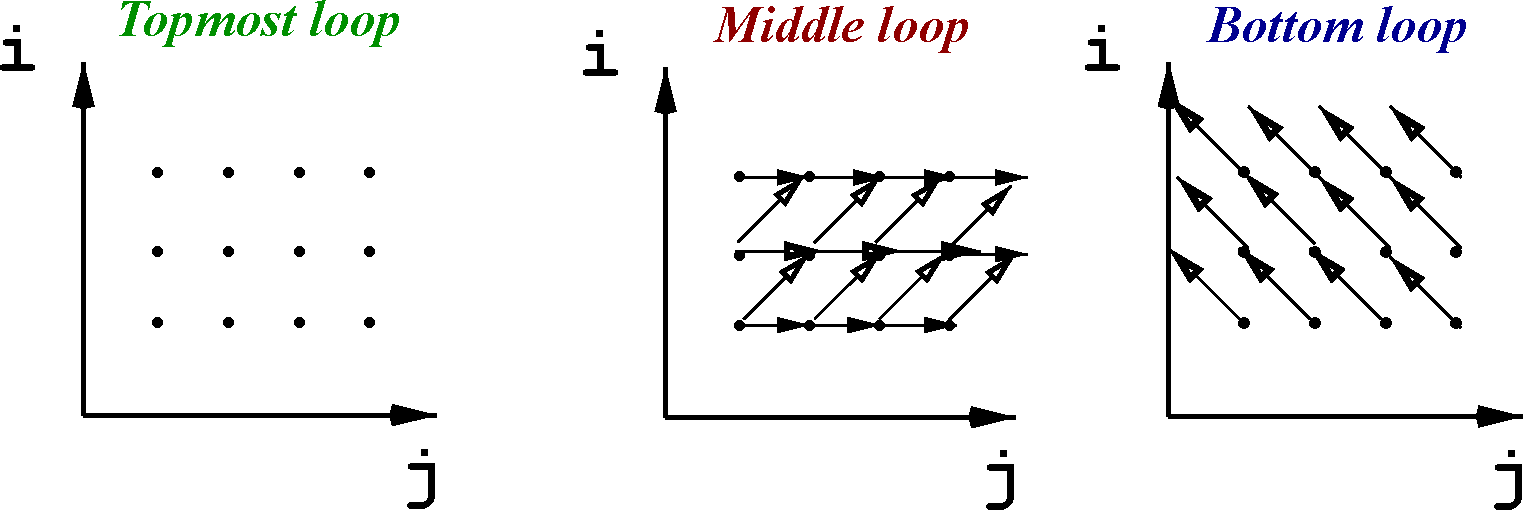
\includegraphics[width=\textwidth]{img/LoopDeps.pdf}
  \caption{Graphical representation of the dependencies for the three running examples shown in \cref{fig:data-dep-running-eg}; the $x$ and $y$ axis correspond to the index of the inner and outer \lstinline{do} loop, respectively.}
  \label{fig:dep-graph}
\end{figure}

A graphical representation of the dependencies of the three running code
examples is shown in \cref{fig:dep-graph}.   They can be intuitively inferred
as follows:
\begin{itemize}
\item For the loop in \cref{fig:data-dep-running-eg-a}, different
  loop-nest iterations $(i_1,j_1)$ and $(i_2,j_2)$ necessarily read
  and write different array elements \texttt{A[$j_1$][$i_1$]} and
  \texttt{A[$j_2$][$i_2$]}.  This is because our assumption is that
  $(i_1,j_1) \neq (i_2,j_2)$, hence it cannot be that both $i_1 = i_2$
  and $j_1 = j_2$. As such, the representation of dependencies should
  be a set of points (no arrows), meaning that all dependencies
  actually occur inside the same iteration---in fact they are anti
  intra-iteration dependencies (WAR) because \texttt{A[j][i]} is read
  first and then \texttt{A[j][i]} is written inside the same
  iteration.
\item For the loop in \cref{fig:data-dep-running-eg-b} we reason
  individually for statements $S_1$ and $S_2$ because each statement
  accesses (one) array \texttt{A} and \texttt{B}, respectively:
  \begin{itemize}
  \item[$S_1:$] Let's take an iteration, say $(i_1=2, j_1=3)$,
    which \emph{reads} element \texttt{A[$j_1$-1][$i_1$-1] = A[2][1]}.
    Since an iteration $(i,j)$ always writes the element
    \texttt{A[i][j]}, we can reason that iteration $(i_2=1, j_2=2)$
    will \emph{write} the same element \texttt{A[2][1]}.
    It follows that we have discovered a true (RAW) dependency,
    depicted in the figure with and arrow, from the source
    iteration $(i_2=1, j_2=2)$---which writes \texttt{A[2][1]}---to
    the sink iteration $(i_1=2, j_1=3)$---which reads \texttt{A[2][1]}.
    This is because iteration $(1,2) < (2,3)$ according to the
    lexicographical ordering, and as such, the read happens after
    the write (RAW) in program order. One can individually reason
    for each point of the iteration space and fill it with oblique,
    forward-pointing arrows denoting true dependencies between
    different instances of statement $S_1$
    (executing in different iterations).
  \item[$S_2:$] Following a similar rationale, iteration $(i_1=2, j_1=3)$
    \emph{reads} element \texttt{B[$j_1$-1][$i_1$] = B[2][2]}, and
    iteration $(i_2=2, j_2=2)$ \emph{writes} element \texttt{B[2][2]}.
    It follows that we have discovered a true (RAW) dependency
    with source $(i_2=2, j_2=2)$ and sink $(i_1=2, j_1=3)$,
    because $(2,2) < (2,3)$ in lexicographic ordering.
    Since $i_1=i_2$ we depict the arrow parallel with the
    horizontal axis (that depicts values of $j$). One can
    fill in the rest of the iteration space with horizontal arrows.
  \end{itemize}

\item For the loop in \cref{fig:data-dep-running-eg-c} we reason in a
  similar way: take iteration $(i_1=2, j_1=3)$ that \emph{reads}
  element \texttt{A[2-1][3+1] = A[1][4]}. This element is
  \emph{written} by iteration $(i_2=1,j_2=4)$. It follows that we have
  discovered a true (RAW) from source $(i_2=1,j_2=4)$ to sink
  $(i_1=2, j_1=3)$---because the read happens in iteration $(2,3)$
  which comes after the write in iteration $(1,4)$, i.e.,
  $(1,4) < (2,3)$.  Thus, one can fill in the iteration space with
  oblique, backward-pointing arrows, denoting true dependencies
  between instances of $S_1$ executing in different iterations.
\end{itemize}

We have applied above a human type of reasoning and, as a result, we
have a graphical representation of all dependencies. However, such a
reasoning is not suitable for automation because (i) the loop counts
are statically unknown---they depend on the dataset---hence one cannot
possibly represent an arbitrary large iteration space, and, more
importantly, (ii) even if the loop counts would be statically known it
is still inefficient to maintain and work with all this pointwise
information.

A representation that promotes automated reasoning should succinctly
capture the repeated pattern in the figure. Intuitively and
imprecisely, for \cref{fig:data-dep-running-eg-a} the pattern would
correspond to a point, for \cref{fig:data-dep-running-eg-b} it would
correspond to two arrows---one oblique and one horizontal forward
pointing arrows---and for \cref{fig:data-dep-running-eg-c} it would
correspond to an oblique, backward-pointing arrow.
%
These patterns are formalized by introducing the notion of
\emph{direction vectors}.

\begin{definition}[Dependency direction vector]\label{Dep-Dir-Vect}

  Assume there exists a dependency with source $S_{1}$ in iteration $\vec{k}$
  to sink $S_{2}$ in iteration $\vec{l}$ ($\vec{k}\leq\vec{l}$).
  We denote by $m$ the depth of the loop nest, we use $i$ to range
  from $0,\ldots,m-1$, and we denote by $x_i$ the $i^{th}$
  element of some vector $\vec{x}$ of length $m$.

  The \emph{direction vector} between the instance of statement $S_1$
  executed in some source iteration $\vec{k}$ and statement $S_2$
  executed in sink iteration $\vec{l}$ is denoted by
  $\vec{D}(S_1\in\vec{k},S_{2}\in\vec{l})$, and corresponds to a vector
  of length $m$, whose elements are defined as:

  \begin{equation}
    D_i(S_1\in\vec{k},S_2\in\vec{l})=
    \begin{cases}
      \mbox{\texttt{<}} \ \ \ \ \mbox{\textrm{if it is provably that}} ~~k_i ~<~ l_i,\\
      \mbox{\texttt{=}} \ \ \ \ \mbox{\textrm{if it is provably that}} ~~k_i ~=~ l_i,\\
      \mbox{\texttt{>}} \ \ \ \ \mbox{\textrm{if it is provably that}} ~~k_i ~>~ l_i,\\
      \mbox{\texttt{{}*}} \ \ \ \ \mbox{\textrm{if}}~k_i ~\mbox{\textrm{{}and}}~ l_i~\mbox{are statically uncomparable.}\\
    \end{cases}
    \label{eqn:dir-vec}
 \end{equation}
\end{definition}

The first three cases of the definition above assume that the ordering
relation between $k_i$ and $l_i$ can be statically derived in a generic
fashion (for any source $k_i$ and $l_i$); if this is not possible than
we use the notation \texttt{*} which \emph{conservatively} assumes that any
directions may be possible---i.e., star should be understood as
simultaneous existence of all \texttt{<, =, >} directions. For example,
the loop
\begin{lstlisting}[mathescape=true]
for (int i = 0; i < N; i++)
  $S_1:$  A[ X[i] ] = ...
\end{lstlisting}
would result in direction vector \texttt{[*]} corresponding to a
potential output dependency (WAW), because the write access to
\texttt{A[ X[i] ]} is statically unanalysable---for example under the
assumption that the index array \texttt{X} is part of the
dataset---and, as such, all direction vectors may possibly hold
between various pairs of instances of statement $S_1$ executed in
different iterations.

Note that the symbols \texttt{<, =, >} are \emph{not} connected at all
to the type of the dependency, e.g., true (RAW) or anti (WAR)
dependency.  The type of the dependency is solely determined by the
operation of the source and that of the sink: If the source is a write
statement and the sink is a read then we have a true (RAW) dependency;
if the source is a read and the sink is a write then we have an anti
(WAR) dependency; if both source and sink are writes then we have an
output (WAW) dependency.

The meaning of the symbol \texttt{>} at some position $i$ is that
the source iteration at loop-level $i$ is greater than the sink
iteration at loop-level $i$. This case is possible, for example
the code in \cref{fig:data-dep-running-eg}(c) shows a dependency
with source iteration $(1,4)$ and sink iteration $(2,3)$. At the
level of the second loop, we have $4 > 3$ hence the direction
is \texttt{>} but still the source iteration is less than the sink
iteration $(1,4) < (2,3)$ because of the first loop level.
This observation leads to the following corollary:

\begin{corollary}[Direction vector legality]\label{Leg-Dir-Vect}

  A direction vector is legal (well formed), if removing the
  \texttt{=} entries does \emph{not} result in a leading \texttt{>}
  symbol, as this would mean that an iteration depends on a future
  iteration, and depending on a future event is considered impossible,
  and as such illegal.
\end{corollary}

It remains to determine the sort of reasoning that can be applied to
compute the direction vectors for the code examples in
\cref{fig:data-dep-running-eg}:
\begin{description}
\item[The loop in \cref{fig:data-dep-running-eg-a}:] dependencies can
  occur only between instances of statement $S_1$, executed in
  different (or the same) iterations.  We recall that, by the
  definition of dependency, the two (dependent) iterations must access
  the same element of \texttt{A} and at least one iteration should
  perform a write.  Since statement $S_1$ performs a read and a write
  to elements of array \texttt{A}, two kinds of dependencies may
  occur:
  \begin{description}
  \item[WAW:] an output dependency may be caused by two write accesses
    in two different iterations, denoted $(i_1,j_1)$ and
    $(i_2,j_2)$. The written element is thus \texttt{A[j$_1$][i$_1$]},
    which must be the same as \texttt{A[j$_2$][i$_2$]} for a
    dependency to exist. By \cref{eqn:dir-vec} this results in the
    system of equations
    \[
      \begin{cases}i_1 = i_2\\j_1 = j_2\end{cases}
    \]
    which leads to direction vector \texttt{[=,=]}.  Hence, an output
    dependency from $S_1$ to $S_1$ happens in the same iteration, but
    statement $S_1$ executes only one write access in the same
    iteration.  The conclusion is that no output dependency can occur,
    hence the direction vector is discarded.
  \item[RAW:] a true or anti dependency---we do not know yet
    which---will be caused by the read access from \texttt{A} and the
    write access to \texttt{A} in different (or same)
    iterations. Remember that a statement such as \texttt{A[j][i] =
      A[j][i] + 3} actually corresponds to three hardware
    instructions, hence either a cross- or an intra-iteration
    dependency will necessarily occur.  Assume some iteration
    $(i_1, j_1)$ reads from \texttt{A[j$_1$][i$_1$]} and iteration
    $(i_2,j_2)$ writes to \texttt{A[j$_2$][i$_2$]}.  In order for a
    dependency to exist, the memory location of the read and write
    must coincide; this results in the system of equations
    \[
      \begin{cases}i_1 = i_2\\j_1 = j_2\end{cases}
    \]
    from which we can derive the direction vector:
    \texttt{[=,=]}. This implies that the dependency happens in the
    same iteration, hence it is an intra-iteration dependency.
    Furthermore, since the write follows the read in the instruction
    order of an iteration, this is an anti dependency (WAR).
  \end{description}

\item[For the loop in \cref{fig:data-dep-running-eg-b}:] dependencies
  may possibly occur between instances of statement $S_1$
  and between instances of statement $S_2$. The case of
  output dependencies is disproved by a treatment similar
  to the bullet above. It remains to examine the dependency
  caused by a read and a write in different instances of
  $S_1$ and $S_2$, respectively:
  \begin{description}
  \item[$S_1$:] assume iteration $(i_1,j_1)$ and iteration $(i_2,j_2)$
    reads from and writes to the same element of \texttt{A},
    respectively. Putting this in \cref{eqn:dir-vec} results in the
    system
    \[
      \begin{cases}i_1-1 = i_2\\j_1-1 = j_2\end{cases}
    \]
    which necessarily means that $i_1 > i_2$ and $j_1 > j_2$.
    However, we do not know yet which iteration is the source and
    which is the sink. Assuming that $(i_1, j_1)$ is the source
    results in the direction vector \texttt{[>,>]}, which is illegal
    by \cref{Leg-Dir-Vect}, because a direction vector cannot start
    with the \texttt{>} symbol. It follows that our assumption was
    wrong: $(i_2, j_2)$ is the source and $(i_1, j_1)$ is the sink,
    which means that this is a cross-iteration true dependency
    (RAW)---because the sink iteration reads the element that was
    previously written by the source iteration---and its direction
    vector is \texttt{[<,<]}.
  \item[$S_2$:] a similar rationale can be applied to
    determine that two instances of $S_2$ generate
    a true cross-iteration dependency (RAW), whose
    direction vector is \texttt{[=,<]}. In short, using the
    same notation results in the system of equations
    \[
      \begin{cases}i_1 = i_2\\j_1-1 = j_2\end{cases}
    \]
    hence the source must be $(i_2,j_2)$ and the sink must be
    $(i_1,j_1)$ and the direction vector is \texttt{[=,<]}.
  \end{description}

\item[For the loop in \cref{fig:data-dep-running-eg-c}:] dependencies
  may possibly occur between instances of statement $S_1$.  Assume
  iteration $(i_1,j_1)$ and $(i_2,j_2)$ reads from and writes to the
  same element of \texttt{A}, respectively.  Putting this into
  \cref{eqn:dir-vec} results in the system
  \[
    \begin{cases}i_1-1 = i_2\\j_1+1 = j_2\end{cases}
  \]
  which necessarily implies that $i_1 > i_2$ and $j_1 < j_2$. Choosing
  $(i_1,j_1)$ as the source of the dependency results in direction
  vector \texttt{[>,<]}, which is illegal because it has \texttt{>} as
  the first non-\texttt{=} outermost symbol, as stated by
  \cref{Leg-Dir-Vect}. It follows that $(i_1,j_1)$ must be the sink
  and $(i_2,j_2)$ must be the source, which results in the direction
  vector \texttt{[<,>]}, which is legal. Since the source writes and
  the sink reads, we have a true dependency (RAW).  Moreover since the
  direction vector indicates that the source iteration is strictly
  less than the sink iteration, this is also a cross-iteration
  dependency.
\end{description}

\begin{definition}[Dependency direction matrix]\label{Dep-Dir-Mat}
  A direction matrix is obtained by stacking together the
  direction vectors of all the intra- and cross-iteration
  dependencies of a loop nest (i.e., between any possible
  pair of write-write or read-read instruction instances).
\end{definition}

In conclusion, the direction matrices for the three running code
examples:

\begin{description}
\item[\Cref{fig:data-dep-running-eg-a}:]
  $\begin{cases}\texttt{[=,=]}\end{cases}$
\item[\Cref{fig:data-dep-running-eg-b}:]
  $\begin{cases}\texttt{[<,<]}\\\texttt{[=,<]}\end{cases}$
\item[\Cref{fig:data-dep-running-eg-c}:]
  $\begin{cases}\texttt{[<,>]}\end{cases}$
\end{description}

The following sections will show how the legality of powerful code
transformations can be reasoned in a simple way in terms of direction
vectors/matrices.

\section{Determining loop parallelism}
\label{sec:loop-par}

A loop is said to be parallel if its execution does not cause any
(true, anti, or output) dependencies between iterations---the loop
execution is assumed to be fixed in a specific iteration of an
(potentially empty) enclosing loop context.

The following theorem states that a sufficient condition for a loop to
be parallel is that for all the elements in the loop's corresponding
direction-matrix column, it holds that the element is either
\texttt{=} or there exists an outer loop whose corresponding direction
is \texttt{<} (on that row).  In the latter case we say that the outer
loop \emph{carries} all the dependencies of the inner loop, i.e.,
fixing an iteration of the outer loop (think executing the outer loop
sequentially) would guarantee the absence of cross-iteration
dependencies in the inner loop.

\begin{theorem}[Parallel loop]\label{Loop-Par}

  We assume a loop nest denoted by $\vec{L}$, whose direction matrix
  is denoted by $M$ and consists of $m$ rows.  A sufficient condition
  for a loop at depth $k$ in $\vec{L}$, denoted $L_k$, to be parallel
  is that $\forall i\in\{0,\ldots m-1\}~$ either $M[i][k]$ is
  \texttt{=} or there exists an outer loop at depth $q<k$ such that
  $M[i][q]$ is \texttt{<}.  Proof left as an exercise.
\end{theorem}

\Cref{Loop-Par} claims to give only a sufficient condition for loop
parallelism because it assumes that symbols such as \texttt{*} may be
part of the direction vector elements---we recall that \texttt{*}
conservatively assumes that all directions \texttt{<,=,>} may be
possible. If \texttt{*} does not appear in the direction matrix, then
the condition becomes \emph{necessary} as well as sufficient.  Let us
analyse the parallelism of each loop in our running examples:

\begin{description}
\item[\Cref{fig:data-dep-running-eg-a}:] The direction matrix is
  \texttt{[=,=]}, hence by \cref{Loop-Par}, both loops in the nest are
  parallel because all the directions are \texttt{=}.

\item[\Cref{fig:data-dep-running-eg-b}:] The direction matrix is
  \[
    M = \begin{cases}\texttt{[<,<]}\\\texttt{[=,<]}\end{cases}
  \]
  hence neither the outer nor the inner loop can be proven parallel by
  \cref{Loop-Par}. In the former case this is because $M[0,0]$ is
  \texttt{<} and there is no other outer loop to carry
  dependencies. In the latter case this is because $M[1,1]$ is
  \texttt{<} and the outer loop for that row has direction \texttt{=}
  (instead of \texttt{<}, which would have been necessary to carry the
  dependencies of the inner loop).

\item[\Cref{fig:data-dep-running-eg-c}:] The direction matrix is
  \texttt{[<,>]}, which means that the outer loop is not
  parallel---because it has a leading \texttt{<} direction---\emph{but
    the inner loop is parallel} because the outer loop starts with
  \texttt{<} on the only row of the direction matrix, and, as such, it
  carries all the dependencies of the inner loop.  To understand what
  this means, take a look again at the actual code in
  \cref{fig:data-dep-running-eg-c}.  Suppose we fix the outer
  iteration number to some value $i$. Then the read accesses always
  refer to row $i-1$ of matrix \texttt{A} and the write accesses
  always refer to row $i$ of \texttt{A}; hence a cross-iteration
  dependency cannot happen in the inner loop because no matter the
  value of $j$, the read and write statement instances cannot possibly
  refer to the same location of \texttt{A}.
\end{description}

%%% Local Variables:
%%% mode: latex
%%% TeX-master: "notes"
%%% End:
